\documentclass{standalone}
\usepackage{tikz}

\newcommand{\mue}{3}
\newcommand{\sta}{1}
\newcommand{\lowX}{0}
\newcommand{\lowY}{0}
\newcommand{\hiX}{5}
\newcommand{\hiY}{0.6}

\begin{document}
    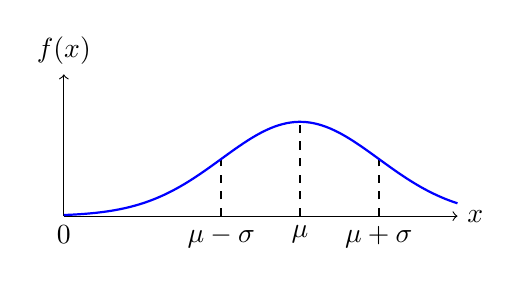
\begin{tikzpicture}[yscale=3]
        
        % Draw the x and y axes
        \draw[->] (\lowX,0) -- (\hiX,0) node[right] {$x$};
        \draw[->] (0,\lowY) -- (0,\hiY) node[above] {$f(x)$};

        % Lines from y=0 to curve
        \draw[black, dashed, thick] (2,0) -- (2,0.24);
        \draw[black, dashed, thick] (\mue,0) -- (\mue,0.4);
        \draw[black, dashed, thick] (4,0) -- (4,0.24);

        % Draw the bell curve
        \draw[scale=1.0,domain=\lowX:\hiX,smooth,variable=\x,blue,thick,samples=100] 
            plot ({\x},{1/(\sta*sqrt(2*pi))*exp(-1/2*((\x-\mue)/\sta)^2)});
        
    
        % Optionally, add labels
        \node[below] at (0,0) {$0$};
        \node[below] at (2,0) {$\mu - \sigma$};
        \node[below] at (\mue,0) {$\mu$};
        \node[below] at (4,0) {$\mu + \sigma$};
    \end{tikzpicture}
\end{document}
